% Don't like 10pt? Try 11pt or 12pt
\documentclass[9pt]{extreport}
%\usepackage[scaled]{helvet}
\renewcommand\familydefault{\sfdefault} 
\usepackage[T1]{fontenc}
%\usepackage{lmodern}
%\usepackage{mathpazo}
\usepackage{kpfonts}
 %\usepackage{mathptmx}
%\setmainfont{uarial}
% This is a helpful package that puts math inside length specifications
\usepackage{calc}
\usepackage[colorlinks,urlcolor=blue]{hyperref}
%\usepackage[pdftex]{graphicx}
\usepackage{graphicx}
\usepackage{wrapfig}
% Simpler bibsection for CV sections
% (thanks to natbib for inspiration)
\makeatletter
\newlength{\bibhang}
\setlength{\bibhang}{1em}
\newlength{\bibsep}
 {\@listi \global\bibsep\itemsep \global\advance\bibsep by\parsep}
\newenvironment{bibsection}%
        {\vspace{-\baselineskip}\begin{list}{}{%
       \setlength{\leftmargin}{\bibhang}%
       \setlength{\itemindent}{-\leftmargin}%
       \setlength{\itemsep}{\bibsep}%
       \setlength{\parsep}{\z@}%
        \setlength{\partopsep}{0pt}%
        \setlength{\topsep}{0pt}}}
        {\end{list}\vspace{-.6\baselineskip}}
\makeatother

% Layout: Puts the section titles on left side of page
\reversemarginpar

%% Use these lines for letter-sized paper
\usepackage[paper=letterpaper,
            %includefoot, % Uncomment to put page number above margin
            marginparwidth=1in,     % Length of section titles
            marginparsep=.09in,       % Space between titles and text
            margin=.6in,               % 1 inch margins
            includemp]{geometry}

%% More layout: Get rid of indenting throughout entire document
\setlength{\parindent}{0in}

%% This gives us fun enumeration environments. compactitem will be nice.
\usepackage{paralist}

\usepackage{fancyhdr,lastpage}
\pagestyle{fancy}
%\pagestyle{empty}      % Uncomment this to get rid of page numbers
\fancyhf{}\renewcommand{\headrulewidth}{0pt}
\fancyfootoffset{\marginparsep+\marginparwidth}
\newlength{\footpageshift}
\setlength{\footpageshift}
          {0.5\textwidth+0.5\marginparsep+0.5\marginparwidth-2in}
\lfoot{\hspace{\footpageshift}%
       \parbox{4in}{\, \hfill %
                    \arabic{page} of \protect\pageref*{LastPage} % +LP
%                    \arabic{page}                               % -LP
                    \hfill \,}}

% Finally, give us PDF bookmarks
\usepackage{color,hyperref}
\definecolor{darkblue}{rgb}{0.0,0.0,0.3}
\hypersetup{colorlinks,breaklinks,
            linkcolor=darkblue,urlcolor=darkblue,
            anchorcolor=darkblue,citecolor=darkblue}

% The title (name) with a horizontal rule under it
%
% Usage: \makeheading{name}
%
% Place at top of document. It should be the first thing.
\newcommand{\makeheading}[1]%
        {\hspace*{-\marginparsep minus \marginparwidth}%
         \begin{minipage}[t]{\textwidth+\marginparwidth+\marginparsep}%
                {\Large \bfseries #1}\\[-0.15\baselineskip]%
                 \rule{\columnwidth}{1pt}%
         \end{minipage}}

\newcommand{\makechapter}[1]%
        {\hspace*{-\marginparsep minus \marginparwidth}%
         \phantomsection\addcontentsline{toc}{section}{#1}%
         \begin{minipage}[t]{\textwidth+\marginparwidth+\marginparsep}%
                %\vspace %
                \vspace{3 mm}
                {\large \bfseries #1}%\\[-0.15\baselineskip]%
                %\vspace{-.4\baselineskip}
                %\rule{\columnwidth}{1pt}%
         \end{minipage}}


% The section headings
%
% Usage: \section{section name}
%
% Follow this section IMMEDIATELY with the first line of the section
% text. Do not put whitespace in between. That is, do this:
%
%       \section{My Information}
%       Here is my information.
%
% and NOT this:
%
%       \section{My Information}
%
%       Here is my information.
%
% Otherwise the top of the section header will not line up with the top
% of the section. Of course, using a single comment character (%) on
% empty lines allows for the function of the first example with the
% readability of the second example.
\renewcommand{\section}[2]%
        {\pagebreak[2]\vspace{0.8\baselineskip}%
         %\phantomsection\addcontentsline{toc}{section}{#1}%
         \hspace{0in}%
         \marginpar{
         \raggedright \emph{#1}}#2}

\newcommand{\ssection}[2]%
        {\pagebreak[2]\vspace{0.3\baselineskip}%
         \hspace{0in}%
         \marginpar{
         \raggedright \emph{#1}}#2}


% An itemize-style list with lots of space between items
\newenvironment{outerlist}[1][\enskip\textbullet]%
        {\begin{itemize}[#1]}{\end{itemize}%
         \vspace{-.4\baselineskip}}

% An environment IDENTICAL to outerlist that has better pre-list spacing
% when used as the first thing in a \section
\newenvironment{lonelist}[1][\enskip\textbullet]%
        {\vspace{-\baselineskip}\begin{list}{#1}{%
        \setlength{\partopsep}{0pt}%
        \setlength{\topsep}{0pt}}}
        {\end{list}\vspace{-.4\baselineskip}}

% An itemize-style list with little space between items
\newenvironment{innerlist}[1][\enskip\textbullet]%
        {\vspace{0.2\baselineskip}\begin{compactitem}[#1]}{\end{compactitem}}

% An environment IDENTICAL to innerlist that has better pre-list spacing
% when used as the first thing in a \section
\newenvironment{loneinnerlist}[1][\enskip\textbullet]%
        {\vspace{-\baselineskip}\begin{compactitem}[#1]}
        {\end{compactitem}\vspace{-.4\baselineskip}}

% To add some paragraph space between lines.
% This also tells LaTeX to preferably break a page on one of these gaps
% if there is a needed pagebreak nearby.
\newcommand{\blankline}{\quad\pagebreak[2]}

% Uses hyperref to link DOI
%\newcommand\doilink[1]{\href{http://dx.doi.org/#1}{#1}}
%\newcommand\doi[1]{doi:\doilink{#1}}


%%%%%%%%%%%%%%%%%%%%%%%% End Helper Commands %%%%%%%%%%%%%%%%%%%%%%%%%%%

%%%%%%%%%%%%%%%%%%%%%%%%% Begin CV Document %%%%%%%%%%%%%%%%%%%%%%%%%%%%

\begin{document}
\makeheading{{\sc \LARGE curriculum vitae} \hfill Duc Tam Hoang}
\begin{wrapfigure}[0]{r}{2.5cm}
\begin{center}
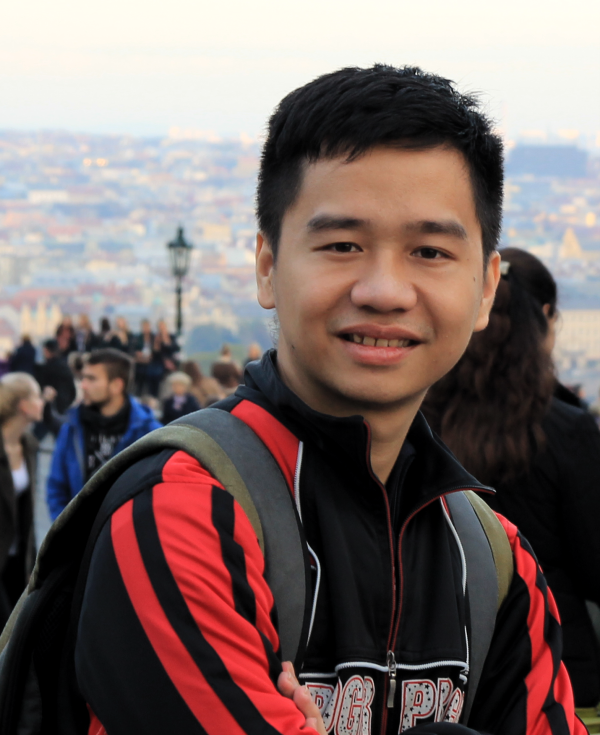
\includegraphics[width=2.5cm]{tamhd_2.png}
\end{center}
\end{wrapfigure}

\makechapter{Contact Information}

\newlength{\rcollength}\setlength{\rcollength}{1.85in}%
%
\section{Name} 
\textbf{Duc Tam Hoang} (or simply \textbf{Tam Hoang})

%\href{http://mff.cuni.cz/}{Mathematics and Physics Faculty, Charles University in Prague}
Computational Linguistics Lab, National University of Singapore

\ssection{Address}
%527, Koleje Otava, Chemick\'a 954, Praha 4, Prague
\# 05-407, Block 117, Lorong 1 Toa Payoh, 310117, Singapore

\ssection{Email}
%\href{mailto:tamhd1990@gmail.com}{tamhd1990@gmail.com}
\href{mailto:hoangdt@comp.nus.edu.sg}{hoangdt@comp.nus.edu.sg}

\ssection{Mobile}
+65 90548590

\ssection{Skype}
tamhd1990

\makechapter{Education}

\section{2013-2015}
%
\textbf{Charles University in Prague} \hfill Czech Republic

\begin{innerlist}

\item[] M.S, Computational Linguistics, Computer Science
        \begin{innerlist}
        %\item Faculty: Mathematics and Physics
		\item Graduate with honors
        \item GPA: 1.07 (\textit{excellent} - equivalent to 3.9 in the US 4.0 scale)
        \item Thesis: Pivoting Vietnamese Machine Translation System
        \end{innerlist}
\end{innerlist}

%\blankline

\section{2008-2012}
\textbf{University of Engineering and Technology, VNU} \hfill Vietnam

\begin{innerlist}

\item[] B.Sc, Computer Science (Honors Program)
        \begin{innerlist}
	%\item Program: International Standard Program
        \item GPA: 3.33/4.00 (\textit{Distinction})
        \item Thesis: \small{An Ontology-based Vietnamese QA System for Academic Regulation}
        \end{innerlist}

\end{innerlist}
\makechapter{Work/Research Experience}

\section{2015-present}
\textbf{National University of Singapore}, Singapore
\begin{innerlist}
    \item[] \textit{Research Assistant}%
    \begin{innerlist}
        \item Topic: Grammatical Error Correction
        \item Task: Read papers, propose solutions, program systems and write reports/papers.
    \end{innerlist}
\end{innerlist}


\section{2014}
\textbf{Institute of Formal and Applied Linguistics}, MFF, UK
\begin{innerlist}
\item[] \textit{Intern}%
    \begin{innerlist}
    \item Topic: Statistical Machine Translation
    \item Task 1: Implement triangulation tools for Moses (Statistical Machine Translation - SMT)   
    \item Task 2: Design SMT homeworks on CodEx
    %\item Advisor: Ond\v{r}ej Bojar (\href{mailto:ondrej.bojar@mff.cuni.cz}{ondrej.bojar@mff.cuni.cz})
    \end{innerlist}
\end{innerlist}


\section{2013-2014}
%
\textbf{TextAn - MFF automatic analysis of Police documents}, Prague

\begin{innerlist}

\item[] \textit{Developer - Software Project - MFF:  \href{https://github.com/PreXident/TextAn}{https://github.com/PreXident/TextAn}} 
 	\begin{innerlist}
     \item Topic: Automatic analysis of human report.
     \item Task: Implement Automatic Object Assigner: mapping natural entity to database object
     \item Sub-task: Implemente a ranking scheme
     \item Sub-task: Integrate Machine Learning Classifier into a Java Project
    \end{innerlist}
\end{innerlist}

\section{2010-2013}
\textbf{Human Machine Interaction Laboratory }, UET/Coltech, VNU
\begin{innerlist}
\item[] \textit{Research Assistant} \hfill In cooperation with Japan Advanced Institute of Science and Technology
    \begin{innerlist}
    \item \textbf{\textit{Topic 1: Question Answering Systems}} (3 separated projects)
    \item Task 1: Design database in MySQL, Ontology OWL from text file
    \item Task 2: Design web interface for QA system
    \item Task 3: Write rules/patterns for Vietnamese questions (in multiple domains)
	\item Task 4: Implement maximum graph matching for tokens and objects.
    \item \textbf{\textit{Topic 2: Information Retrieval System}}
    \item Task 1: Crawl data from forums and teachnical websites
    \item Task 2: Integrate cluster tool and search tools into project
    \end{innerlist}
\end{innerlist}
\vspace{.4\baselineskip}
\begin{innerlist}
\item[] \textit{Teaching Assistant} %\textit{Assistant Lecturer}%
 	\begin{innerlist}
     \item Teaching Fundamental Informatics: C/C++ Programming
     \item Teaching Mathematics Team for the 21$^{st}$ Vietnam Mathematics Olympiad for Undergraduates, 2013.
     %\item Tutor students during office hours and lab sections, graded  weekly lab reports, graded exams and assignments.
    \end{innerlist}
\end{innerlist}


\section{2011}
\textbf{Presentation Club}, UET, VNU
\begin{innerlist}
\item[] \textit{Organizer of club's meetings and events} %\textit{Assistant Lecturer}%
\end{innerlist}

\makechapter{Research Interests}
\begin{innerlist}
\item[] \textit{I am interested in topics of Computational Linguistics} %\textit{Assistant Lecturer}%
\end{innerlist}

\makechapter{Background/Skills}
%
\begin{innerlist}
\item Background: Mathematics, Computational Linguistics, Computer Science.
\item Programming Languages: {\bf Python}, Perl, Shell/Bash Script, Java, C/C++.
\item Tools: Git, Svn, MySQL, Lucene, Carrot$^2$, Moses (inc. eman/ems)
\item Others: Regular Expression, Dynamic Programming, Object-oriented Programming, CSS/HTML/JSP. 
\item Favourite Editor: vim
\end{innerlist}

\makechapter{Language Proficiency} 
%
\begin{innerlist}
\item Vietnamese - native
\item English - fluent
\item Czech - basic
\end{innerlist}

\makechapter{Awards \& Honors}
%

\section{2014}
\textbf{Excellence Scholarship} for top Students at Faculty of Mathematics and Physics, Charles University in Prague.
\vspace{-.6\baselineskip}
\section{2013}
\textbf{Fully-funded master scholarship} at Charles University in Prague. %{\scriptsize \textit{So far, I have been the only one who ever won this scholarship}}

\vspace{-.6\baselineskip}

\section{2010-2012}
\textbf{1 First prize and 2 Second prizes} at Vietnamese National Mathematical Olympiad for Undergraduates.

Several \textbf{Young Symbolization} awards at University of Engineering and Technology.

\textbf{Government Fellowship} for excellent students in the ISP program.

\textbf{Excellent Academic Performance} at UET/Coltech.

Rank \textbf{1$^{st}$} at the University Entrance Exam of UET/Coltech, VNU.



\makechapter{Publications}

\textbf{Conference papers}
\begin{enumerate}

\item[4.] \underline{Duc Tam Hoang}, Ond\v{r}ej Bojar. \textbf{TmTriangulate: A Tool for Phrase-Table Triangulation}. The Prague Bulletin of Mathematical Linguistics, 2015.

\item[3.] Tung Xuan Vu, Minh Le Nguyen, \underline{Duc Tam Hoang}. \textbf{Semantic Parsing for Vietnamese Question Answering System}. The 7th international conference on Knowledge and Systems Engineering, Vietnam, 2015.

\item[2.] \underline{Duc Tam Hoang}, Minh Le Nguyen, Son Bao Pham. \textbf{L2S: Transforming natural language questions to SQL queries}. The 7th international conference on Knowledge and Systems Engineering, Vietnam, 2015.

\item[1.] Dat Tien Nguyen, \underline{Duc Tam Hoang}, Son Bao Pham. \textbf{A Vietnamese Natural Language Interface to Database}[\href{http://ieeexplore.ieee.org/xpl/articleDetails.jsp?reload=true&arnumber=6337095}{PDF}]. Sixth IEEE International Conference on Semantic Computing September 19-21, 2012 Palermo, Italy
\end{enumerate}

\newpage

\makechapter{References} 
\section{upon request}
%
Prof. NG Hwee Tou	

School of Computing, National University of Singapore

13 Computing Drive, Singapore 117417

Telephone: (+65) 6516 8951

Email: \href{mailto:nght@comp.nus.edu.sg}{nght@comp.nus.edu.sg}

Homepage: \href{https://www.comp.nus.edu.sg/$\sim$nght/}{https://www.comp.nus.edu.sg/$\sim$nght/}
%

RNDr. Ond\v{r}ej Bojar, Ph.D.

Institute of Formal and Applied Linguistics, Charles University in Prague

Malostranske namesti 25, 118 00 Praha 1, Czech Republic

Telephone: (+420) 221 914 276

Email: \href{mailto:ondrej.bojar@mff.cuni.cz}{ondrej.bojar@mff.cuni.cz}

Homepage: \href{http://www1.cuni.cz/~obo/}{http://www1.cuni.cz/$\sim$obo/} \\
%

Assoc. Prof., Dr. Son Bao Pham 

Dean of Faculty of Information Technology

University of Engineering and Technology, Vietnam National University, Hanoi

Room 316, E3 Building, 144 Xuan Thuy, Cau Giay, Hanoi

Telephone: (+84) 936413663

Email: \href{mailto:sonpb@vnu.edu.vn}{sonpb@vnu.edu.vn}

Homepage: \href{http://coltech.vnu.edu.vn/\~sonpb/}{http://coltech.vnu.edu.vn/$\sim$sonpb/} \\ 

\bigskip


%%(Under request)

%%\begin{center}

%%\tiny{Last updated: July 2012}
%%\end{center}


\end{document}

%%%%%%%%%%%%%%%%%%%%%%%%%% End CV Document %%%%%%%%%%%%%%%%%%%%%%%%%%%%%
